%!TEX program = xelatex
\documentclass[dvipsnames, svgnames,a4paper,11pt]{article}
% ----------------------------------------------------- 
%	加边框的命令
%	参考:https://tex.stackexchange.com/questions/531559/how-to-add-the-page-border-for-first-two-pages-in-latex
\usepackage{tikz}
\usetikzlibrary{calc}
\usepackage{eso-pic}
\AddToShipoutPictureBG{%
\begin{tikzpicture}[overlay,remember picture]
\draw[line width=0.6pt] % 边框粗细
    ($ (current page.north west) + (0.6cm,-0.6cm) $)
    rectangle
    ($ (current page.south east) + (-0.6cm,0.6cm) $); % 边框位置
\end{tikzpicture}}


\usepackage{xcolor}
\definecolor{c1}{HTML}{070F94} % 目录颜色 原版为2752C9 紫灰色535AAA 蓝紫色0B0DB7 深蓝色070F94 湖绿色219394 松石灰绿086173
\definecolor{c2}{HTML}{E20129} % 引用颜色 原版\definecolor{c2}{RGB}{190,20,83} 橙色F24729

\usepackage{ctex}
\usepackage[top=28mm,bottom=28mm,left=15mm,right=15mm]{geometry}
\usepackage{hyperref} 
\hypersetup{
	colorlinks,
	linktoc = section, % 超链接位置,选项有section, page, all
	linkcolor = c1, % linkcolor 目录颜色
	citecolor = c1  % citecolor 引用颜色
}
\usepackage{amsmath,enumerate,multirow,float}
\usepackage{tabularx}
\usepackage{tabu}
\usepackage{subfig}
\usepackage{fancyhdr}
\usepackage{graphicx}
\usepackage{wrapfig}  
\usepackage{physics}
\usepackage{appendix}
\usepackage{amsfonts}

%
\usepackage{tcolorbox}
\tcbuselibrary{skins,breakable}
\newtcolorbox{tbox}[2][]{
    colframe=black!70!,
    breakable,
    enhanced,
	boxrule =0.5pt,
    title = {#2},
    fonttitle = \large\kaishu\bfseries,
	drop fuzzy shadow,
    #1
}
\newtcolorbox[auto counter,number within=section]{question}[1][]{
  top=2pt,bottom=2pt,arc=1mm,
  boxrule=0.5pt,
%   frame hidden,
  breakable,
  enhanced, %跨页后不会显示下边框
  coltitle=c1!80!gray,
  colframe=c1,
  colback=c1!3!white,
  drop fuzzy shadow,
  title={思考题~\thetcbcounter:\quad},
  fonttitle=\bfseries,
  attach title to upper,
  #1
}

% ---------------------------------------------------------------------
%	利用cleveref改变引用格式,\cref是引用命令
\usepackage{cleveref}
\crefformat{figure}{#2{\textcolor{c2}{Figure #1}}#3} % 图片的引用格式
\crefformat{equation}{#2{(\textcolor{c2}{#1})}#3} % 公式的引用格式
\crefformat{table}{#2{\textcolor{c2}{Table #1}}#3} % 表格的引用格式


% ---------------------------------------------------------------------
%	页眉页脚设置
\fancypagestyle{plain}{\pagestyle{fancy}}
\pagestyle{fancy}
\lhead{\kaishu 中山大学物理与天文学院基础物理实验\uppercase\expandafter{\romannumeral2}} % 左边页眉,学院 + 课程
\rhead{\kaishu 实验报告By黄罗琳} % 右边页眉,实验报告标题
\cfoot{\thepage} % 页脚,中间添加页码


% ---------------------------------------------------------------------
%	对目录、章节标题的设置
\renewcommand{\contentsname}{\centerline{\huge 目录}}
\usepackage{titlesec}
\usepackage{titletoc}
% \titleformat{章节}[形状]{格式}{标题序号}{序号与标题间距}{标题前命令}[标题后命令]
\titleformat{\section}{\centering\LARGE\songti}{}{1em}{}

% ---------------------------------------------------------------------
%   listing代码环境设置
\usepackage{listings}
\lstloadlanguages{python}
\lstdefinestyle{pythonstyle}{
backgroundcolor=\color{gray!5},
language=python,
frameround=tftt,
frame=shadowbox, 
keepspaces=true,
breaklines,
columns=spaceflexible,                   
basicstyle=\ttfamily\small, % 基本文本设置,字体为teletype,大小为scriptsize
keywordstyle=[1]\color{c1}\bfseries, 
keywordstyle=[2]\color{Red!70!black},   
stringstyle=\color{Purple},       
showstringspaces=false,
commentstyle=\ttfamily\scriptsize\color{green!40!black},%注释文本设置,字体为sf,大小为smaller
tabsize=2,
morekeywords={as},
morekeywords=[2]{np, plt, sp},
numbers=left, % 代码行数
numberstyle=\it\tiny\color{gray}, % 代码行数的数字字体设置
stepnumber=1,
rulesepcolor=\color{gray!30!white}
}




% ---------------------------------------------------------------------
%	其他设置
\def\degree{${}^{\circ}$} % 角度
\graphicspath{{./images/}} % 插入图片的相对路径
\allowdisplaybreaks[4]  %允许公式跨页 
\usepackage{lipsum}
\usepackage{adjustbox}
%\usepackage{mathrsfs} % 字体
%\captionsetup[figure]{name=Figure} % 图片形式
%\captionsetup[table]{name=Table} % 表格形式
\begin{document}
	
	% 实验报告封面	
	% 顶栏
	\begin{table}
		\renewcommand\arraystretch{1.7}
		\begin{tabularx}{\textwidth}{
				|X|X|X|X
				|X|X|X|X|}
			\hline
			\multicolumn{2}{|c|}{预习报告}&\multicolumn{2}{|c|}{实验记录}&\multicolumn{2}{|c|}{分析讨论}&\multicolumn{2}{|c|}{总成绩}\\
			\hline
			\LARGE25 & & \LARGE25 & & \LARGE30 & & \LARGE80 & \\
			\hline
		\end{tabularx}
	\end{table}
	% ---
	
	% 信息栏
	\begin{table}
		\renewcommand\arraystretch{1.7}
		\begin{tabularx}{\textwidth}{|X|X|X|X|}
			\hline
			年级、专业: & 2022级 物理学 &组号: &实验组1 \\
			\hline
			姓名: &   黄罗琳 & 学号: &22344001   \\
			\hline
			实验时间: & 2024/3/28 & 教师签名: & \\
			\hline
		\end{tabularx}
	\end{table}
	% ---
	
	% 大标题
	\begin{center}
		\LARGE CC1 \quad 热辐射的测量

	\end{center}
	% ---
	
	% 注意事项
	
	% 基本
	\textbf{【实验报告注意事项】}
	\begin{enumerate}
		\item 实验报告由三部分组成:
		\begin{enumerate}
			\item 预习报告:课前认真研读实验讲义,弄清实验原理;实验所需的仪器设备、用具及其使用、完成课前预习思考题;了解实验需要测量的物理量,并根据要求提前准备实验记录表格(可以参考实验报告模板,可以打印)。\textcolor{red}{\textbf{(20分)}}
			\item 实验记录:认真、客观记录实验条件、实验过程中的现象以及数据。实验记录请用珠笔或者钢笔书写并签名(\textcolor{red}{\textbf{用铅笔记录的被认为无效}})。\textcolor{red}{\textbf{保持原始记录,包括写错删除部分,如因误记需要修改记录,必须按规范修改。}}(不得输入电脑打印,但可扫描手记后打印扫描件);离开前请实验教师检查记录并签名。\textcolor{red}{\textbf{(30分)}}
			\item 数据处理及分析讨论:处理实验原始数据(学习仪器使用类型的实验除外),对数据的可靠性和合理性进行分析;按规范呈现数据和结果(图、表),包括数据、图表按顺序编号及其引用;分析物理现象(含回答实验思考题,写出问题思考过程,必要时按规范引用数据);最后得出结论。\textcolor{red}{\textbf{(30分)}}
		\end{enumerate}
		\textbf{实验报告就是将预习报告、实验记录、和数据处理与分析合起来,加上本页封面。\textcolor{red}{(80分)}}
		\item 每次完成实验后的一周内交\textbf{实验报告}(特殊情况不能超过两周)。
	
	\end{enumerate}
	
	% 安全
	\textbf{【实验安全注意事项】}	
	\begin{itemize}
		\item 实验过程中,禁止触摸辐射体表面,一方面是避免在高温时烫伤;另一方面避免污染表面,影响发射系数。
		\item 测量不同辐射表面对辐射强度影响时,辐射温度不要设置太高,更换辐射体时,应带手套。
		\item 实验过程中,计算机在采集数据时不要触摸测试架,以免造成对传感器的干扰。
		\item 在使用控温程序时,要留意程序是否正常运行,若运行有问题,请及时关闭可编程直流电源的输出,防止辐射器温度过高而损坏。停止运行程序时,要用程序的Stop output按钮,不要用菜单键的红色强制终止按钮。
		\item 辐射传感器上方有一块金属挡板。在测量时将挡板移开;非测量时关上,避免不必要的触碰污染传感器表面。
	  \end{itemize}
	
	% 目录
	\clearpage
	\tableofcontents
	\clearpage
	% ---
	
	
	
	% 预习报告	
	
	% 小标题 
	\setcounter{section}{0}
	\section{CC1 热辐射的测量 \quad\heiti 预习报告}
	% ---
	
	% 实验目的
	\subsection{实验目的}
	\begin{enumerate}
	\item 认识热辐射现象及其本质(普遍存在的一种能量转换与传递的形式)。
	\item 认识影响热辐射强度的各种因素及其与热辐射强度的定量关系,包括:辐射体表面温度、辐射距离、表面的发射系数等。
	\item 了解热辐射传感器(SMTIR9902)原理和结构、使用(含校正)方法。
	\item 学习应用LabView管理由具有NI通信协议的非NI专业仪器(数字多用表)、设备(程控电源)构成的实验系统。

	\end{enumerate}
	% ---
	
	% 仪器用具
	\subsection{仪器用具}
	\begin{table}[htbp]
		\centering
		\renewcommand\arraystretch{1.6}
\begin{tabular}{|c|c|c|c|}
\hline
\text{编号} & \text{仪器用具名称} & \text{数量} & \text{主要参数} \\
\hline
1 & \text{黑体辐射与红外测量装置} & 1 & \text{DHRH-B: 含带标尺、位移导轨、辐射器、热辐射传感} \\
\hline
2 & \text{数字多用表} & 2 & \text{RIGOL DM3058E} \\
\hline
3 & \text{程控电源} & 1 & \text{RIGOL DP831} \\
\hline
4 & \text{计算机} & 1 & \text{已安装 LabView 和控温软件} \\
\hline
\end{tabular}
	\end{table}
	% ---
	
	% 原理概述
	\subsection{原理概述}
	\begin{enumerate}
		\item 热辐射是物体由于温度而发出的电磁波现象,是热量传递的一种方式之一。温度高于绝对零度的物体都会产生热辐射,温度越高,辐射总能量越大,短波成分也越多。热辐射的光谱是连续的,波长范围从0到无穷,主要包括波长较长的可见光和红外线。由于电磁波的传播无需介质,热辐射是在真空中唯一的传热方式。
    
    \item 热辐射的特点包括:任何温度高于0K的物体都会不断地向周围空间发出热辐射;它可以在真空和空气中传播;伴随能量形式的转变;具有强烈的方向性;辐射能与温度和波长有关;发射辐射取决于温度的4次方。
    
    \item 热辐射的强度和频率分布与辐射体的温度和性质有关。如果辐射体对电磁波的吸收和辐射达到平衡,则热辐射的特性将只取决于温度,与其他特性无关,称为平衡辐射。
    
    \item 测量热辐射的原理是利用物体对电磁波的吸收、反射和透射等特性来确定物体的温度、表面积、黑度等参数。黑度是指物体吸收单位波长间隔内的辐射通量与入射到该物体的辐射通量之比。黑度越大,说明物体吸收和辐射能力越强,反之则越弱。
    
    \item 实验中,能量的传递过程包括:加热装置将电能转化为热能;辐射体将热能转化为辐射能;传感器将辐射能转化为热能。
    
    \item 辐射器包含加热装置和控温装置。加热装置通过连接到直流电源的陶瓷加热片进行加热;控温装置中,PT1000温度传感器可实时测量辐射体的温度,并通过PID温控系统对辐射体进行温度控制。
    
    \item 辐射传感器由热电偶串联组成,其中热电偶的热端接收辐射能,冷端与传感器外壳相连。当吸热面吸收热量时,热端温度升高,热电偶两端产生温度差,从而产生电势差。因此,辐射通量越大,温差越大,输出电压越大。SMTIR9902的输出信号与当地从辐射方向进入的辐射强度或能流密度成正比。
	\end{enumerate}
	% ---
	
	
	
	% 实验前思考题
	\subsection{实验思考题题}
	
	% 思考题1
	\begin{question}
		人体热辐射会对 SMTIR9902 系列传感器读数产生影响(自己可验证),如何消除这种影响?日光灯是否有影响呢?这种传感器是否适合测量高温热辐射,为什么?
	\end{question}
	人体的一部分能量以电磁波的形式散射出体表,其中大部分为红外线。这些红外线的能量在人体热量散发中起着关键作用,被称为人体红外辐射。\\
日光灯的光谱主要集中在可见光范围内,且距离传感器较远,其影响和忽略不计。因此,在使用SMTIR9902系列传感器时,通常不需要考虑日光灯的光谱对传感器的影响。\\
 SMTIR9902系列传感器的传感器温度范围是-20°C到100°C。如果超出这个范围,传感器将会受到损坏。因此,在应用中需要注意确保传感器的工作温度在这个范围内,以防止传感器损坏。\\
	% 思考题2
	\begin{question}
		如果对辐射体制冷,使辐射表面温度低于室温(传感器温度),辐射传感器输出信号会如何变化?
	\end{question}
	如果对辐射体进行制冷,使其辐射表面的温度低于室温(传感器温度),传感器将不再向外辐射,而是会吸收来自环境中其他物体的辐射。因此,传感器接收到的净红外辐射强度会减小,进而导致输出信号减小。这种情况下,传感器的响应将受到制冷影响,需要考虑这一因素在内,以确保传感器能够正常工作并提供准确的测量数据。
	% 思考题3
	\begin{question}
		按辐射定律,处于室温的物体也有辐射,为何辐射传感器的输出信号为零?如果要直接测量该物体的辐射强度(辐射传感器输出信号正比于辐射强度),环境(传感器外壳)温度应该多高? 如果环境(传感器外壳)温度维持在室温附近但温度有变化, 是否可以通过数学方法扣除(非绝对零度的)环境温度的影响?(对给定辐射源温度, 传感器外壳温度与辐射传感器读数之间是什么关系? 提示,热辐射传感器内置Ni1000可以测量外壳的温度,其分度表见附录2)
	\end{question}

	处于室温的物体与传感器温度相同,二者发出的红外辐射也相同,因此传感器接收到的净红外辐射强度就为零,即辐射传感器的输出信号为零。为了使得传感器能够检测到物体的红外辐射,需要使环境(传感器外壳)的温度低于物体的温度。这样,物体就会向环境发射净红外辐射,而不是吸收净红外辐射。通过数学方法,可以扣除(非绝对零度的)环境温度的影响,以便更准确地测量物体的红外辐射强度。
	\begin{question}
		辐射体的加热功率与辐射体温度之间呈何关系?与辐射传感器的信号值之间呈何关系?为什么?
	\end{question}
	由斯特藩-玻尔兹曼定律可知:$R_T = \sigma T^4$,即辐射体的加热功率与辐射体温度的四次方成正比。这意味着随着温度的升高,辐射体释放的热量迅速增加。\\

	对于辐射传感器,其工作原理是通过测量接收到的辐射功率来获取目标物体的温度。辐射传感器输出的信号值与接收到的辐射功率成正比,即:信号值正比于加热功率正比于$T^{4}$。
	
	
	% ---
	
	
	
	% 实验记录	
	\clearpage
	
	% 顶栏
	\begin{table}
		\renewcommand\arraystretch{1.7}
		\centering
		\begin{tabularx}{\textwidth}{|X|X|X|X|}
			\hline
			专业: & 物理学 & 年级: & 2022级 \\
			\hline
			姓名: & 黄罗琳 & 学号: & 22344001\\
			\hline
			室温: & 25℃ & 实验地点: & A515 \\
			\hline
			学生签名:&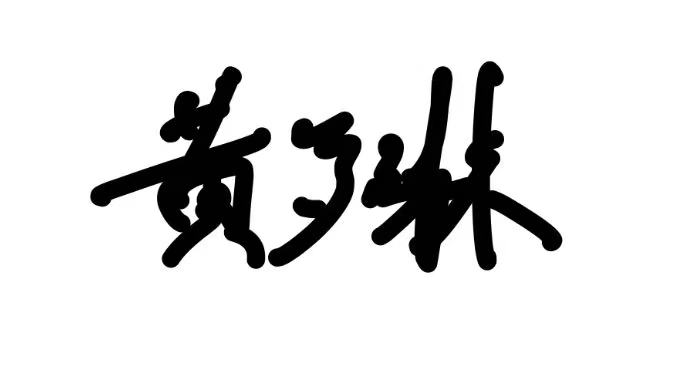
\includegraphics[width=1cm]{签字.jpg}  & 评分: &\\
			\hline
			实验时间:& 2024/3/28 & 教师签名:&\\
			\hline
		\end{tabularx}
	\end{table}
	% ---
	
	% 小标题
	\section{CC1 热辐射的测量 \quad\heiti 实验记录}
	% ---
	
	% 实验过程记录
	\subsection{实验内容、步骤与结果}
	
	%
	\subsubsection{实验系统搭建}
	\begin{enumerate}
		\item 辐射体的安装。辐射体固定于辐射架的最上端,轻旋旁边
		的固定螺丝,即可从上方取下辐射体.\textbf{实验中所有分实验均选取黑面样品进行测量。}
		\item 连接控制系统与数据采集系统。
		\item 检查好所有连线已经正确连接、两台数字万用表、程控电源与电脑通信都正常后,打开“CC1热辐射实验控温程序”。
		\item \textbf{本实验报告中所有数据分析及思考题回答见数据分析部分}
		\begin{figure}[{H}]
			\centering
			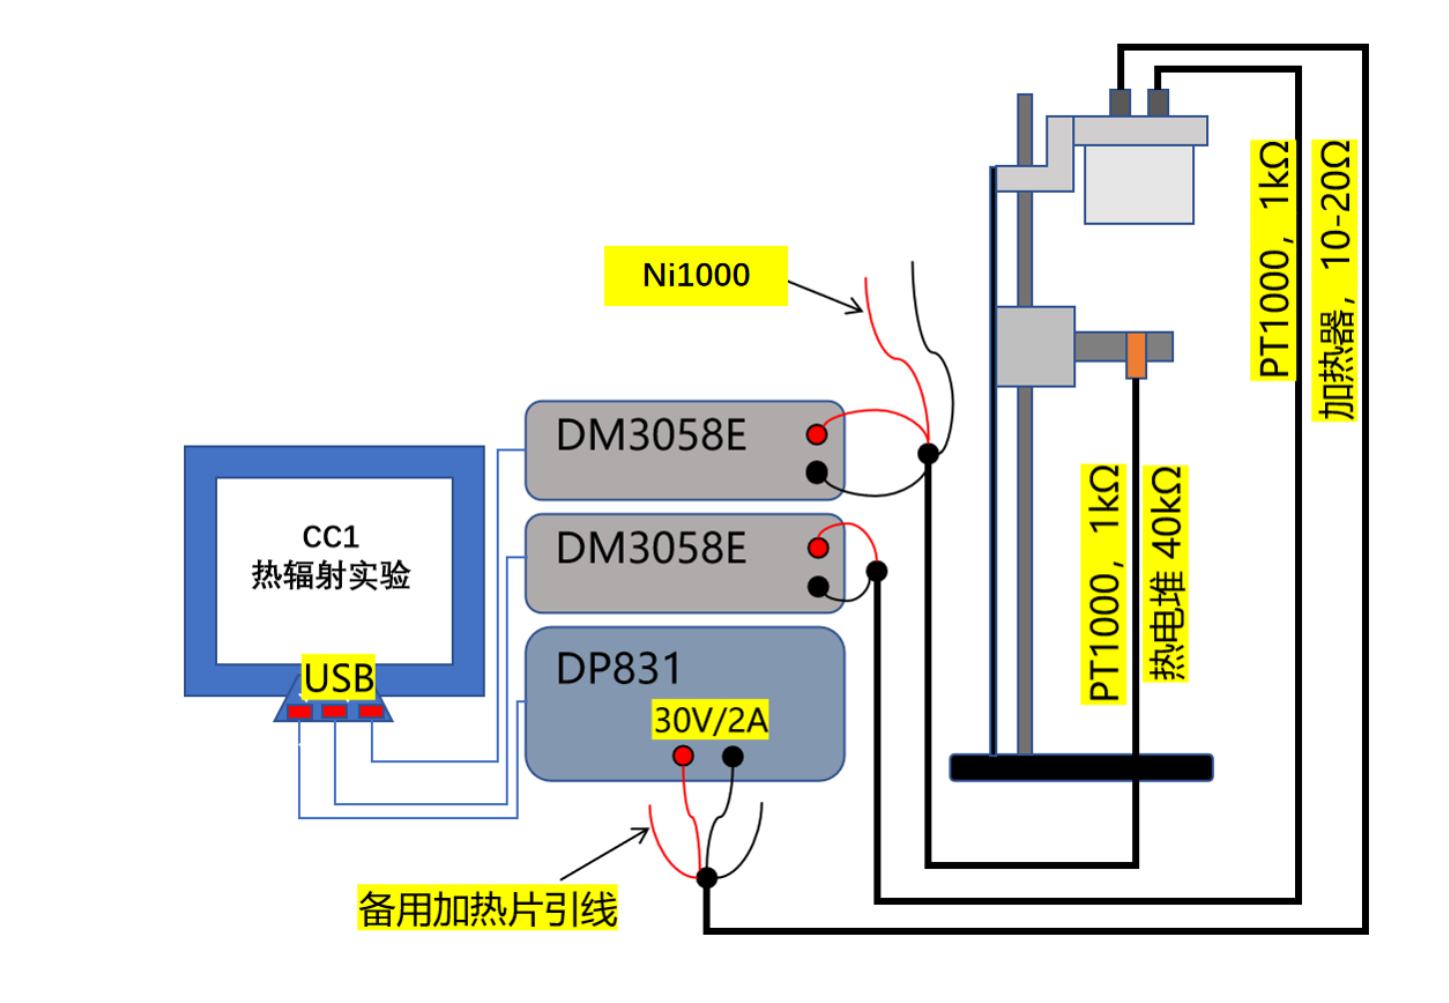
\includegraphics[width=0.4\linewidth]{接线.png}
			\caption{实验仪器接线示意图}
			\label{}
		\end{figure}
		\begin{figure}[{H}]
			\centering
			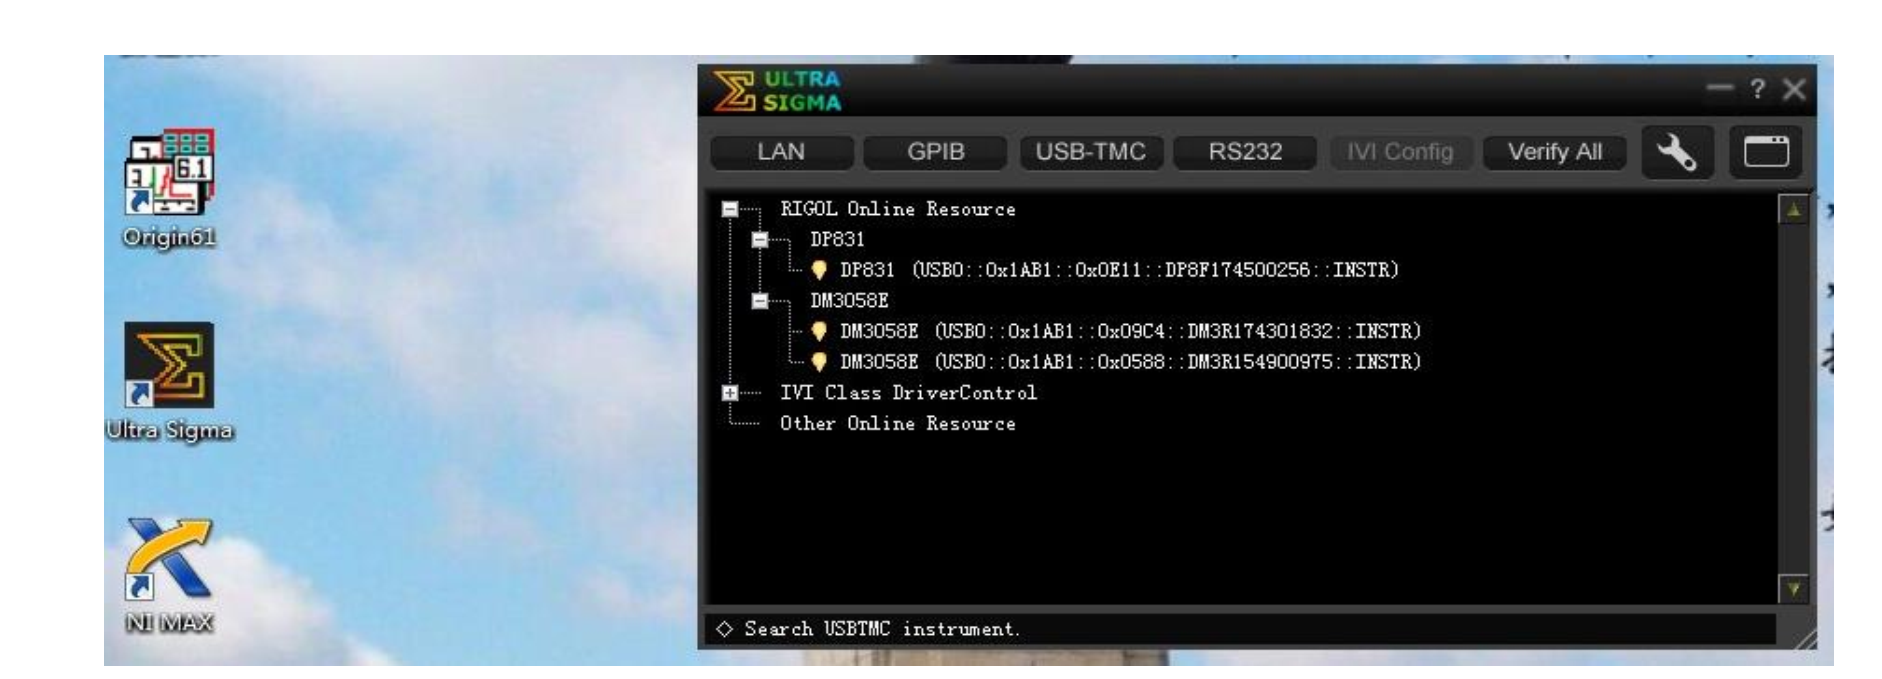
\includegraphics[width=0.3\linewidth]{仪器判断.png}
			\caption{判断是否连接成功(使用软件Ultra
			Sigma)}
			\label{}
		\end{figure}
		\begin{figure}[{H}]
			\centering
			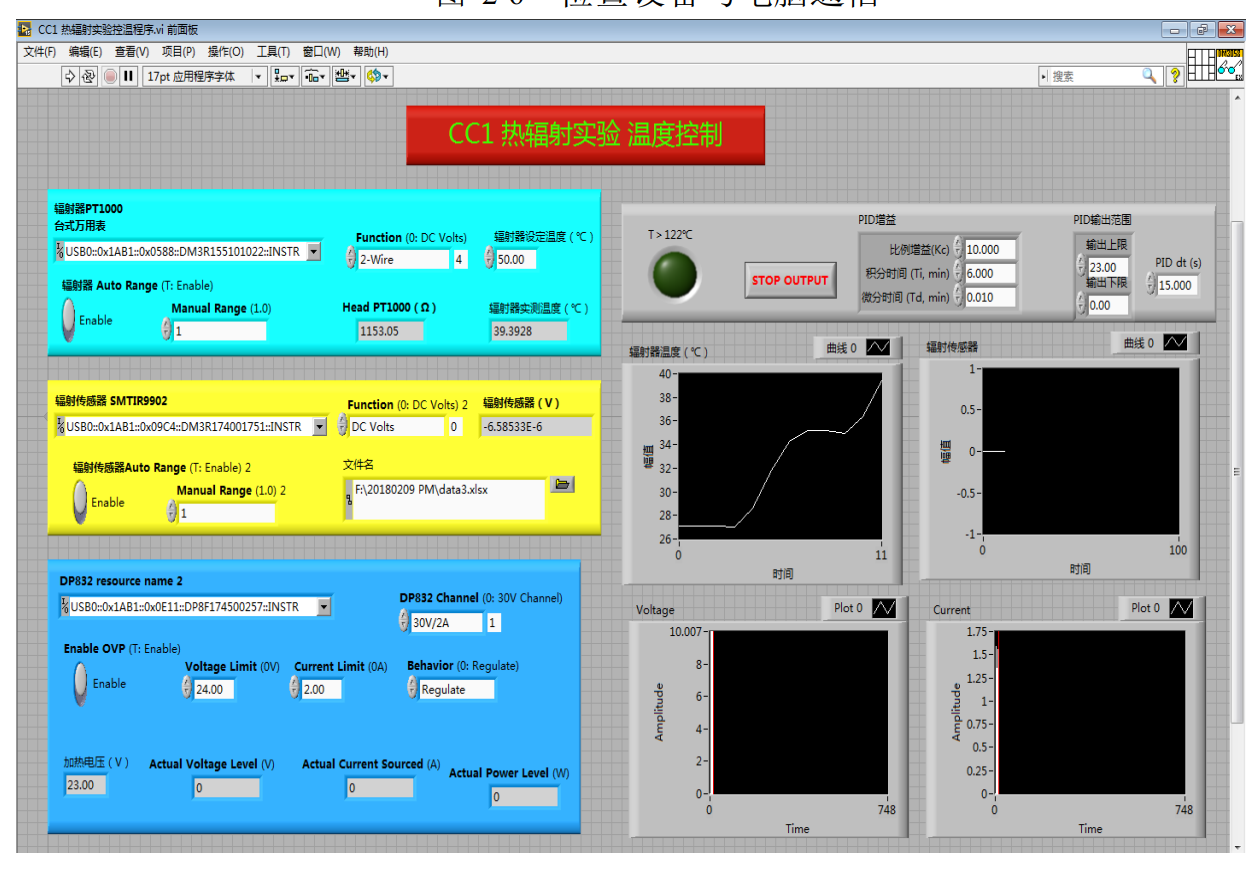
\includegraphics[width=0.3\linewidth]{程序.png}
			\caption{控温程序示例}
			\label{}
		\end{figure}
	\end{enumerate}
	 
	%
	\subsubsection{测量物体的辐射面温度对辐射强度大小的影响}
	\begin{enumerate}
		\item 选择辐射距离为\textbf{150mm},将辐射传感器调至该距离;
		\item 设计5个温度控制点;由于120\textdegree C的断电保护控制,建议设计的控温温度设置值不高于118\textdegree C。记录每个控温点(稳定后)所需的电功率以及辐射传感器输出电压;\\
		  本人学号为001结尾,故选用41\textdegree C开始的五个温度控制点,得到如下数据:
		  \begin{table}[h]
			\centering
			\begin{tabular}{|c|c|c|c|}
			\hline
			设定温度/℃ & 实测温度/℃ & 辐射传感器 & 输出功率(W) \\ \hline
			41          & 40.9463     & 158         & 0.627         \\ \hline
			51          & 50.9856     & 276         & 1.243         \\ \hline
			61          & 60.9884     & 404         & 1.645         \\ \hline
			71          & 70.9994     & 555         & 2.032         \\ \hline
			81          & 80.9907     & 709         & 2.543         \\ \hline
			\end{tabular}
			\caption{实验数据}
			\label{tab:temperature_power_data}
			\end{table}
		\item 分析数据,探索辐射强度与辐射表面温度之间的关系,并绘制温度-辐射强度曲线图;
		\item 分析数据,探索电源加热功率与辐射表面温度之间的关系。\textbf{数据处理见后}
	\end{enumerate}

	\subsubsection{测量在不同辐射距离在d的辐射传感器输出P }
\begin{enumerate}
	\item 将控温度控制目标设置温度$T=89.00^\circ$C,依然选择用光面辐射体进行实验。

\item 设计5个位置测量点。

\item 移动红外传感器的位置,每移动一定的距离后,记录测得对应辐射强度,绘制$P-d^{-2}$图。\\
\textbf{ 本人学号为001结尾,故选用151mm开始的6个位置测量点,得到如下数据}
\begin{table}[htbp]
	\centering
	\caption{不同辐射距离在d的辐射传感器输出P}
	  \begin{tabular}{|c|cccccc|}
		\hline
	  目标距离 $d$ (mm) & 151 & 171 & 191 & 211 & 231&251 \\
	  \hline
	  输出电压 $P$ ($\mu V$ ) & 407 & 282 & 224& 174 & 147&119 \\
	  \hline
	  \end{tabular}%
	\label{tab:data_horizontal}%
  \end{table}%
\end{enumerate}
\subsubsection{测量不同物体表面的发射系数}
将热辐射传感器移开,更换所需辐射面的辐射体。分别正确连接辐射器PT1000和陶瓷加热器的连线到万用表和可编程直流电源上,控温表设置在61℃,待温度控制好后,将热辐射传感器移至靠近辐射体处,测量并记录该辐射传感器读数(实验时,保证热辐射传感器与待测辐射面距离相同(150mm),便于分析和比较)
\begin{table}[H]
	\centering
	\caption{不同表面条件下的辐射传感器输出电压}
	  \begin{tabular}{|c|c|c|c|}
		\hline
	  表面条件 & 黑面 & 粗糙面 & 光面 \\
	  \hline
	  辐射传感器输出电压 $P$ ($\mu V$) & 408 & 157 & 140 \\
	  \hline
	  \end{tabular}%
	\label{tab:data_horizontal}%
  \end{table}%
  \subsubsection{实验数据图像}
  此图像均为实验过程中个温度控制点(41\textdegree C开始的五个温度控制点)的温控程序简化图像
  \begin{figure}[H]
    \centering
    \begin{minipage}[b]{0.23\linewidth}
        \centering
        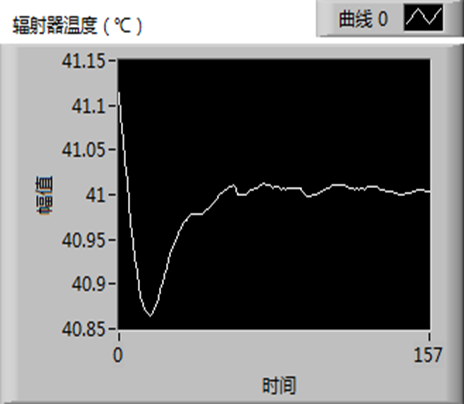
\includegraphics[width=\linewidth]{41-1}
        \caption{辐射器温度}
    \end{minipage}
    \hfill
    \begin{minipage}[b]{0.23\linewidth}
        \centering
        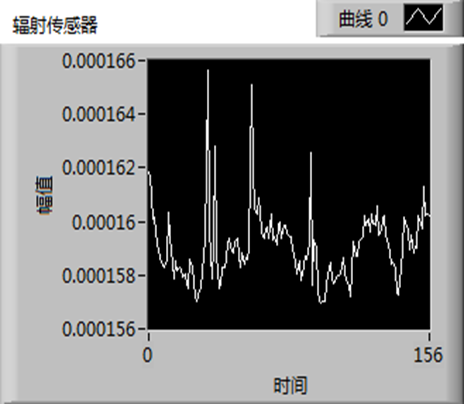
\includegraphics[width=\linewidth]{41-2}
        \caption{传感器示数}
    \end{minipage}
    \hfill
    \begin{minipage}[b]{0.23\linewidth}
        \centering
        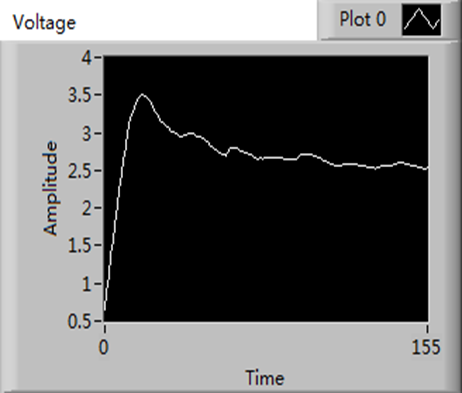
\includegraphics[width=\linewidth]{41-3}
        \caption{电压}
    \end{minipage}
    \hfill
    \begin{minipage}[b]{0.23\linewidth}
        \centering
        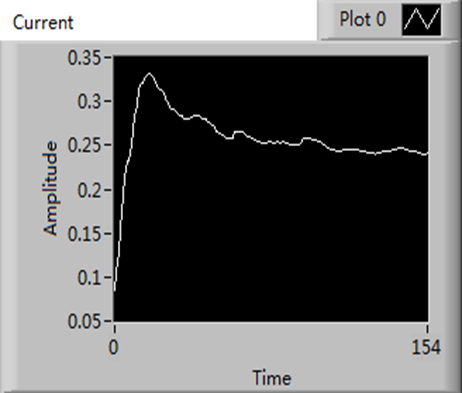
\includegraphics[width=\linewidth]{41-4}
        \caption{电流}
    \end{minipage}
\end{figure}
\begin{figure}[H]
    \centering
    \begin{minipage}[b]{0.23\linewidth}
        \centering
        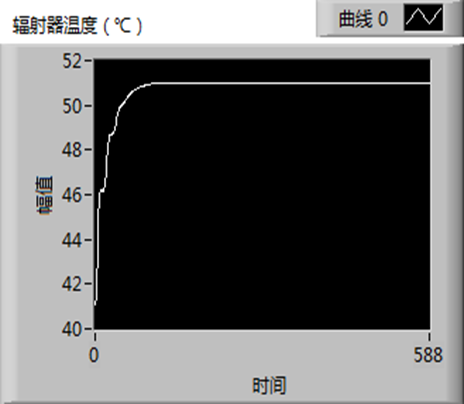
\includegraphics[width=\linewidth]{51-1}
        \caption{辐射器温度}
    \end{minipage}
    \hfill
    \begin{minipage}[b]{0.23\linewidth}
        \centering
        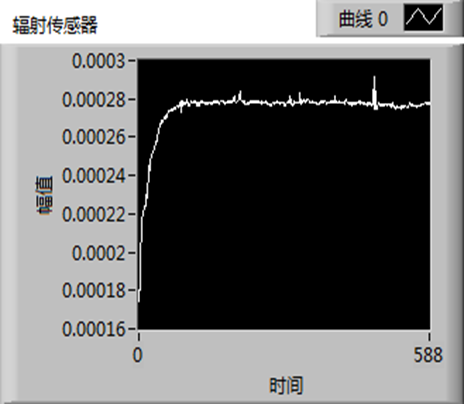
\includegraphics[width=\linewidth]{51-2}
        \caption{传感器示数}
    \end{minipage}
    \hfill
    \begin{minipage}[b]{0.23\linewidth}
        \centering
        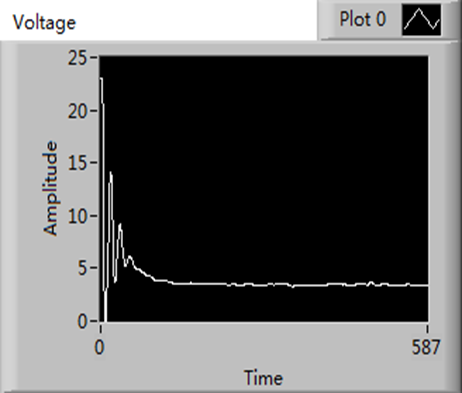
\includegraphics[width=\linewidth]{51-3}
        \caption{电压}
    \end{minipage}
    \hfill
    \begin{minipage}[b]{0.23\linewidth}
        \centering
        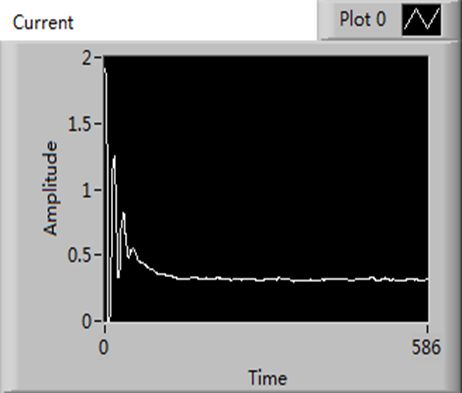
\includegraphics[width=\linewidth]{51-4}
        \caption{电流}
    \end{minipage}
\end{figure}

\begin{figure}[H]
    \centering
    \begin{minipage}[b]{0.23\linewidth}
        \centering
        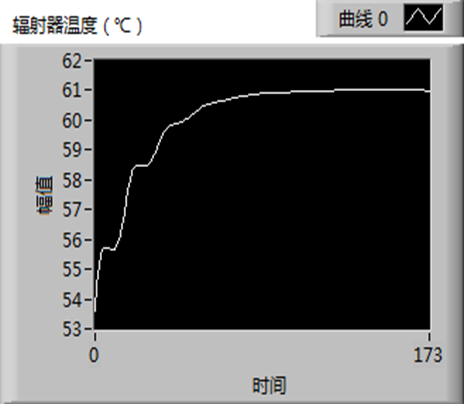
\includegraphics[width=\linewidth]{61-1}
        \caption{辐射器温度}
    \end{minipage}
    \hfill
    \begin{minipage}[b]{0.23\linewidth}
        \centering
        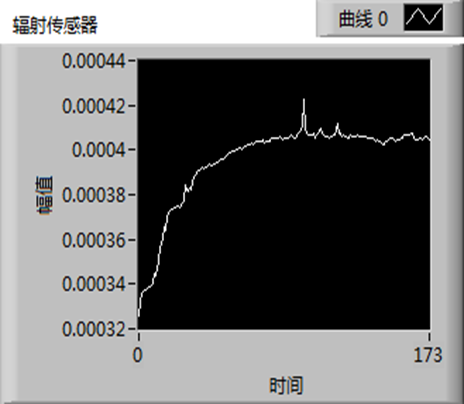
\includegraphics[width=\linewidth]{61-2}
        \caption{传感器示数}
    \end{minipage}
    \hfill
    \begin{minipage}[b]{0.23\linewidth}
        \centering
        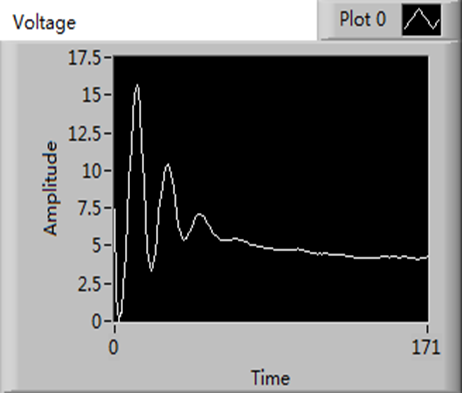
\includegraphics[width=\linewidth]{61-3}
        \caption{电压}
    \end{minipage}
    \hfill
    \begin{minipage}[b]{0.23\linewidth}
        \centering
        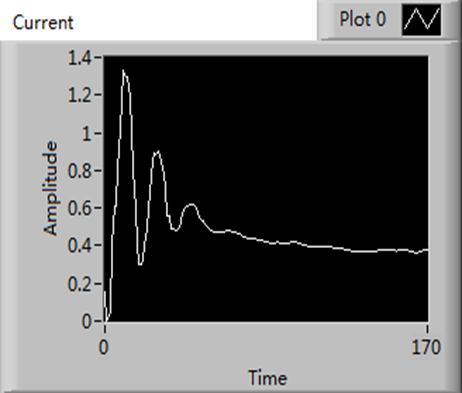
\includegraphics[width=\linewidth]{61-4}
        \caption{电流}
    \end{minipage}
\end{figure}
\begin{figure}[H]
    \centering
    \begin{minipage}[b]{0.23\linewidth}
        \centering
        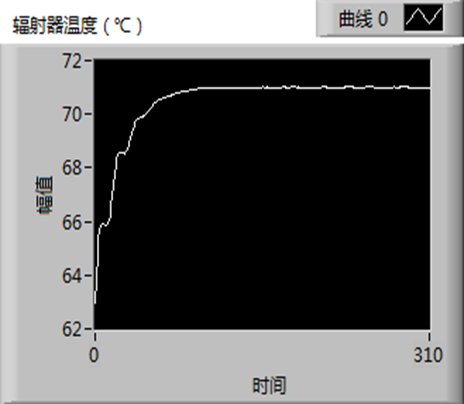
\includegraphics[width=\linewidth]{71-1}
        \caption{辐射器温度}
    \end{minipage}
    \hfill
    \begin{minipage}[b]{0.23\linewidth}
        \centering
        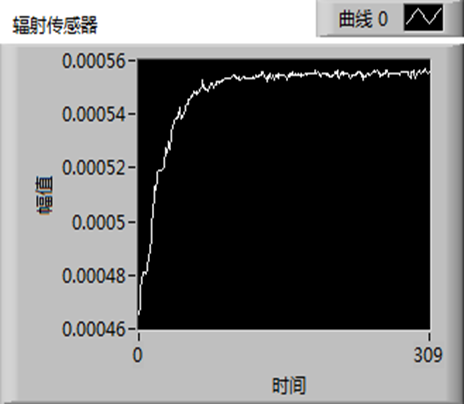
\includegraphics[width=\linewidth]{71-2}
        \caption{传感器示数}
    \end{minipage}
    \hfill
    \begin{minipage}[b]{0.23\linewidth}
        \centering
        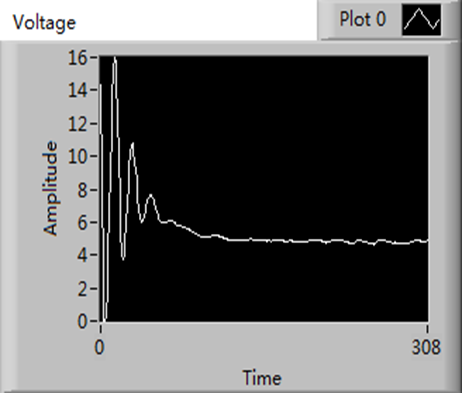
\includegraphics[width=\linewidth]{71-3}
        \caption{电压}
    \end{minipage}
    \hfill
    \begin{minipage}[b]{0.23\linewidth}
        \centering
        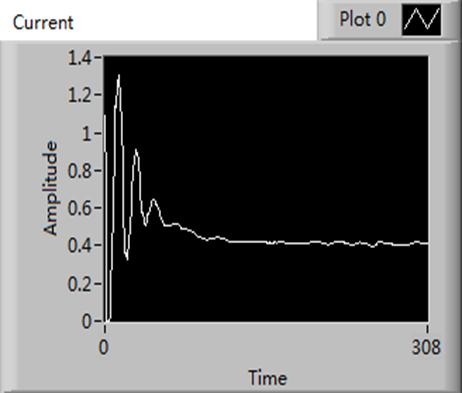
\includegraphics[width=\linewidth]{71-4}
        \caption{电流}
    \end{minipage}
\end{figure}

% Repeat similar code blocks for 81 and 91 with appropriate filenames

\begin{figure}[H]
    \centering
    \begin{minipage}[b]{0.23\linewidth}
        \centering
        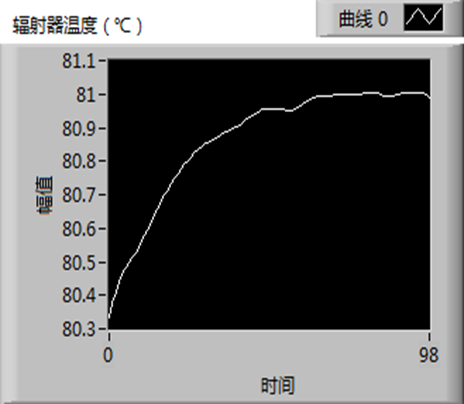
\includegraphics[width=\linewidth]{81-1}
        \caption{辐射器温度}
    \end{minipage}
    \hfill
    \begin{minipage}[b]{0.23\linewidth}
        \centering
        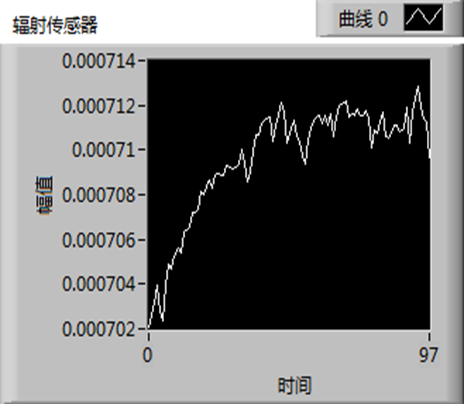
\includegraphics[width=\linewidth]{81-2}
        \caption{传感器示数}
    \end{minipage}
    \hfill
    \begin{minipage}[b]{0.23\linewidth}
        \centering
        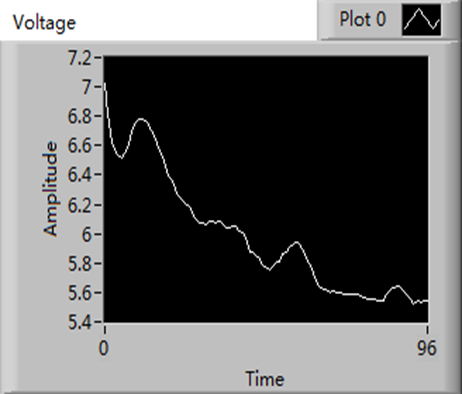
\includegraphics[width=\linewidth]{81-3}
        \caption{电压}
    \end{minipage}
    \hfill
    \begin{minipage}[b]{0.23\linewidth}
        \centering
        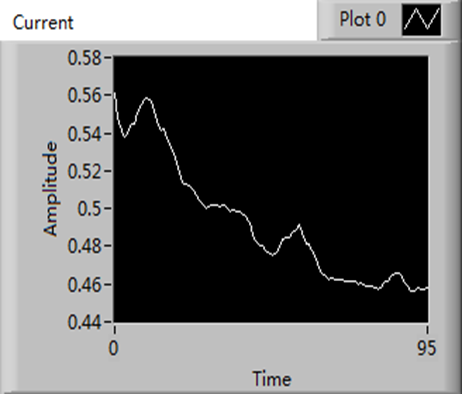
\includegraphics[width=\linewidth]{81-4}
        \caption{电流}
    \end{minipage}
\end{figure}

	\subsection{实验过程遇到问题及解决办法}
	\begin{enumerate}
		\item 首先在接线过程中我出现了接线错误导致的仪器无法正确识别,电脑上温度控制软件无法识别出我所连接的仪器,通过改正接线后,成功正确连接。
		\item 实验中我是通过测量电阻的方式来检查实验仪器的接线,因为实验仪器是无法通过接线口的颜色来判断的,所以需要对内阻进行测量,才能判断是否连接正确。
		\item 实验仪器的各个辐射体有共地的情况,所以在测量之前需要对辐射体是否“共地”进行判断,同样是通过测内阻的方式,例如需要将测量内阻为$0\Omega$ 和$40\Omega$的两组接头分类开来,我的实验仪器上便是黑与黑一组,红与红一组。
		\item 实验中存在我需要调整高度,但是转轴一旦转动会存在无法自行停止的情况,需要用手扶着,我是在同学的帮助下完成了不同高度的实验数据记录。
	\end{enumerate}
	% ---
	
	
	
	% 分析与讨论	
	\clearpage
	
	% 顶栏
	\begin{table}
		\renewcommand\arraystretch{1.7}
		\begin{tabularx}{\textwidth}{|X|X|X|X|}
			\hline
			专业:& 物理学 &年级:& 2022级\\
			\hline
			姓名: & 黄罗琳 & 学号:& 22344001\\
			\hline
			日期:& 2024/3/28 & 评分: &\\
			\hline
		\end{tabularx}
	\end{table}
	% ---
	
	% 小标题
	\section{CC1 热辐射的测量 \quad\heiti 分析与讨论}
	% ---
	
	% 数据处理
	\subsection{实验数据分析}
	
	%
	\subsubsection{测量物体的辐射面温度对辐射强度大小的影响}
	\begin{enumerate}
		\item 实验选取黑面样品进行测量,设定距离为150mm,处理实验数据如下,并绘制拟合曲线如图24所示,拟合曲线横轴为开氏温度的四次方,纵轴为辐射传感器示数。
		\begin{table}[H]
			\centering
			\caption{辐射传感器示数相对于表面温度(开氏度)数据}
			\begin{tabular}{|l|l|l|l|l|l|}
			\hline
				\textbf{设定温度/℃} & 41 & 51 & 61 & 71 & 81  \\ \hline
				\textbf{实测温度/℃} & 40.9463 & 50.9856 & 60.9884 & 70.9994 & 80.9907  \\ \hline
				\textbf{开氏度/K} & 313.9463 & 323.9856 & 333.9884 & 343.9994 & 353.9907   \\ \hline
				\textbf{辐射传感器} & 158 & 276 & 404 & 555 & 709  \\ \hline
				电源输出功率 (W) & 0.627 & 1.243 & 1.645 & 2.032 & 2.543 \\\hline
			\end{tabular}
		\end{table}
		\begin{figure}[{H}]
			\centering
			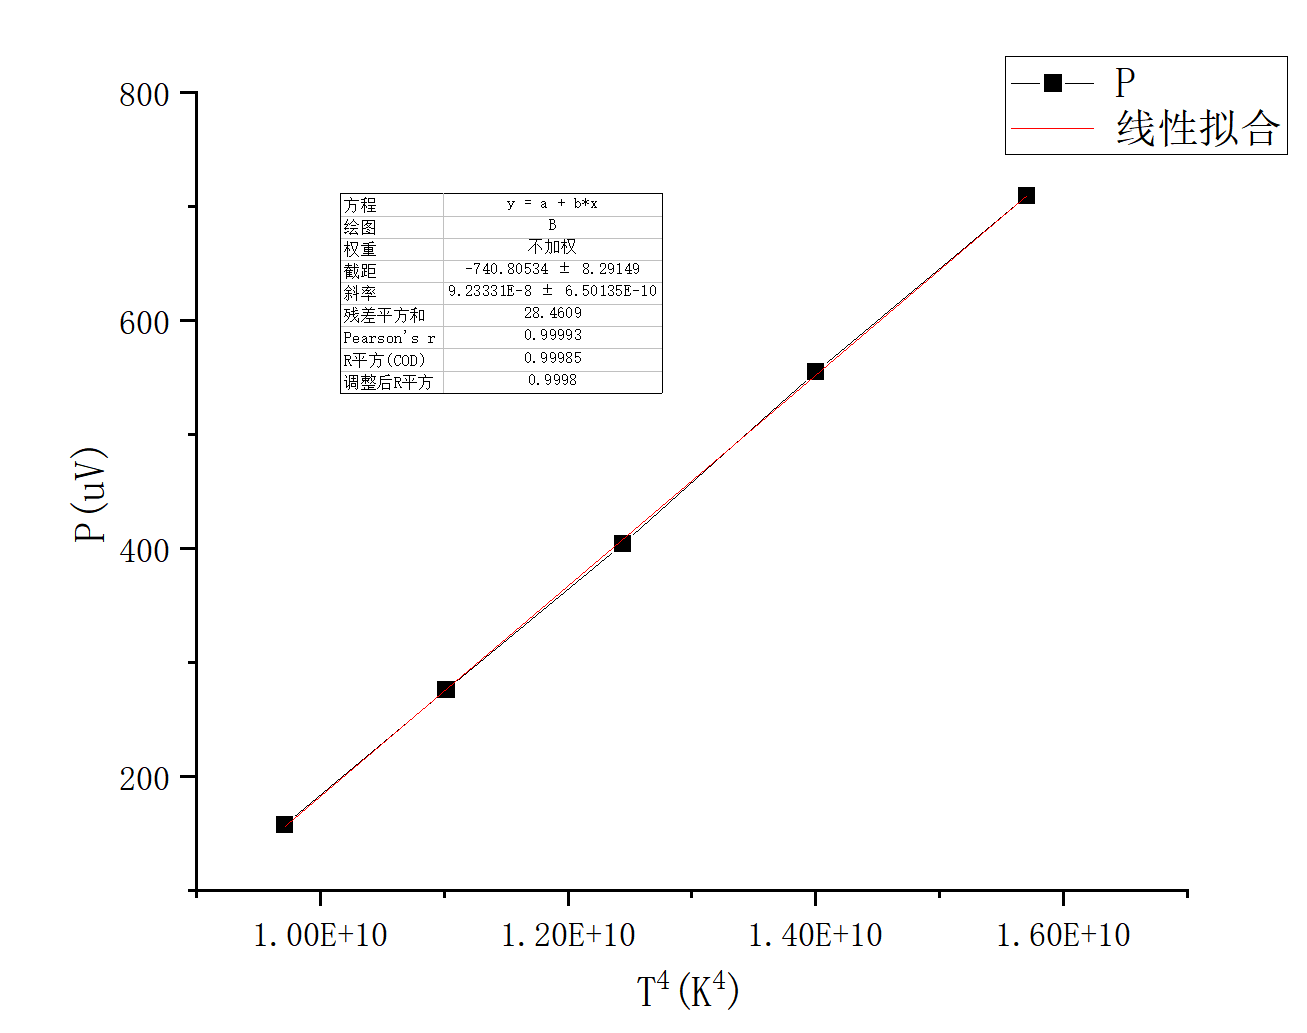
\includegraphics[width=0.6\linewidth]{温度线性拟合.png}
			\caption{辐射传感器示数相对于表面温度$T^4$拟合曲线}
		\end{figure}
	\indent 根据软件导出数据后,得到如下所示的各个数据表,通过分析可知,当温度稳定后,由于仪器精度问题,辐射传感器示数基本处于不变状态,所以只需采用一组代表性数据即可完成所有数据的拟合,故图24的拟合曲线符合实验数据要求和实验原理。
\begin{figure}[{H}]
	\centering
	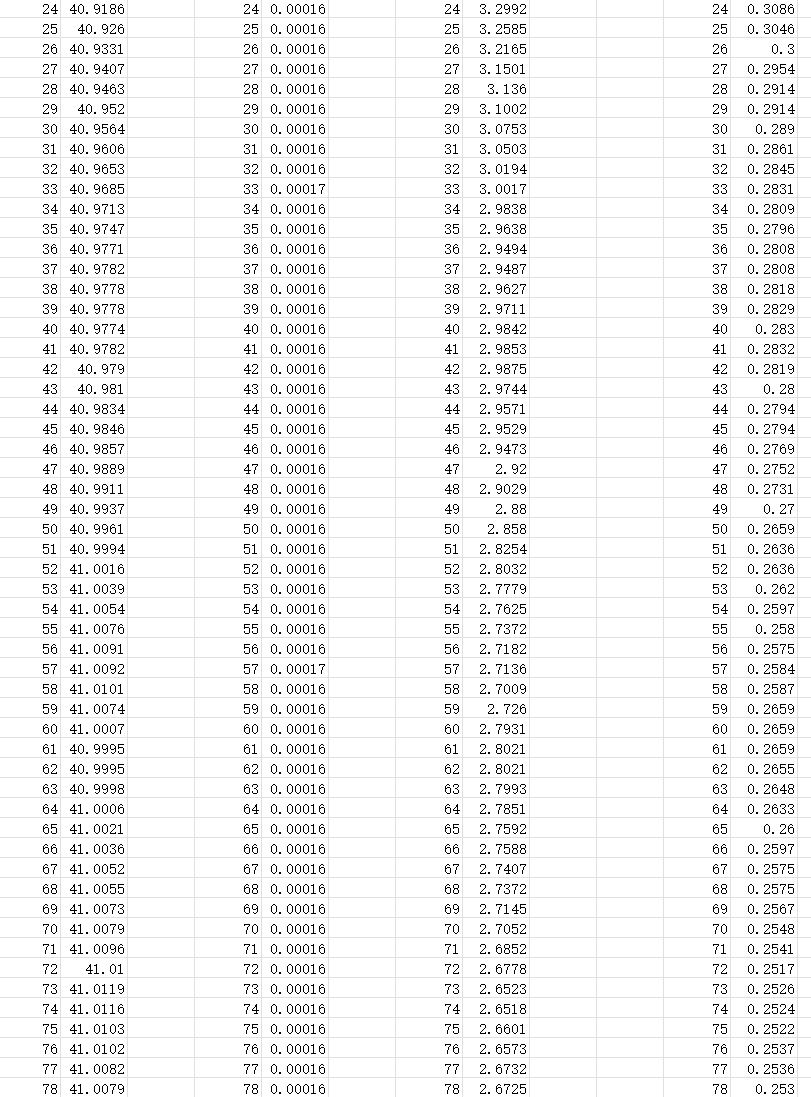
\includegraphics[width=0.4\linewidth]{大量数据1.png}
	\caption{软件数据导出示例}
	\label{}
\end{figure}
\begin{figure}[{H}]
	\centering
	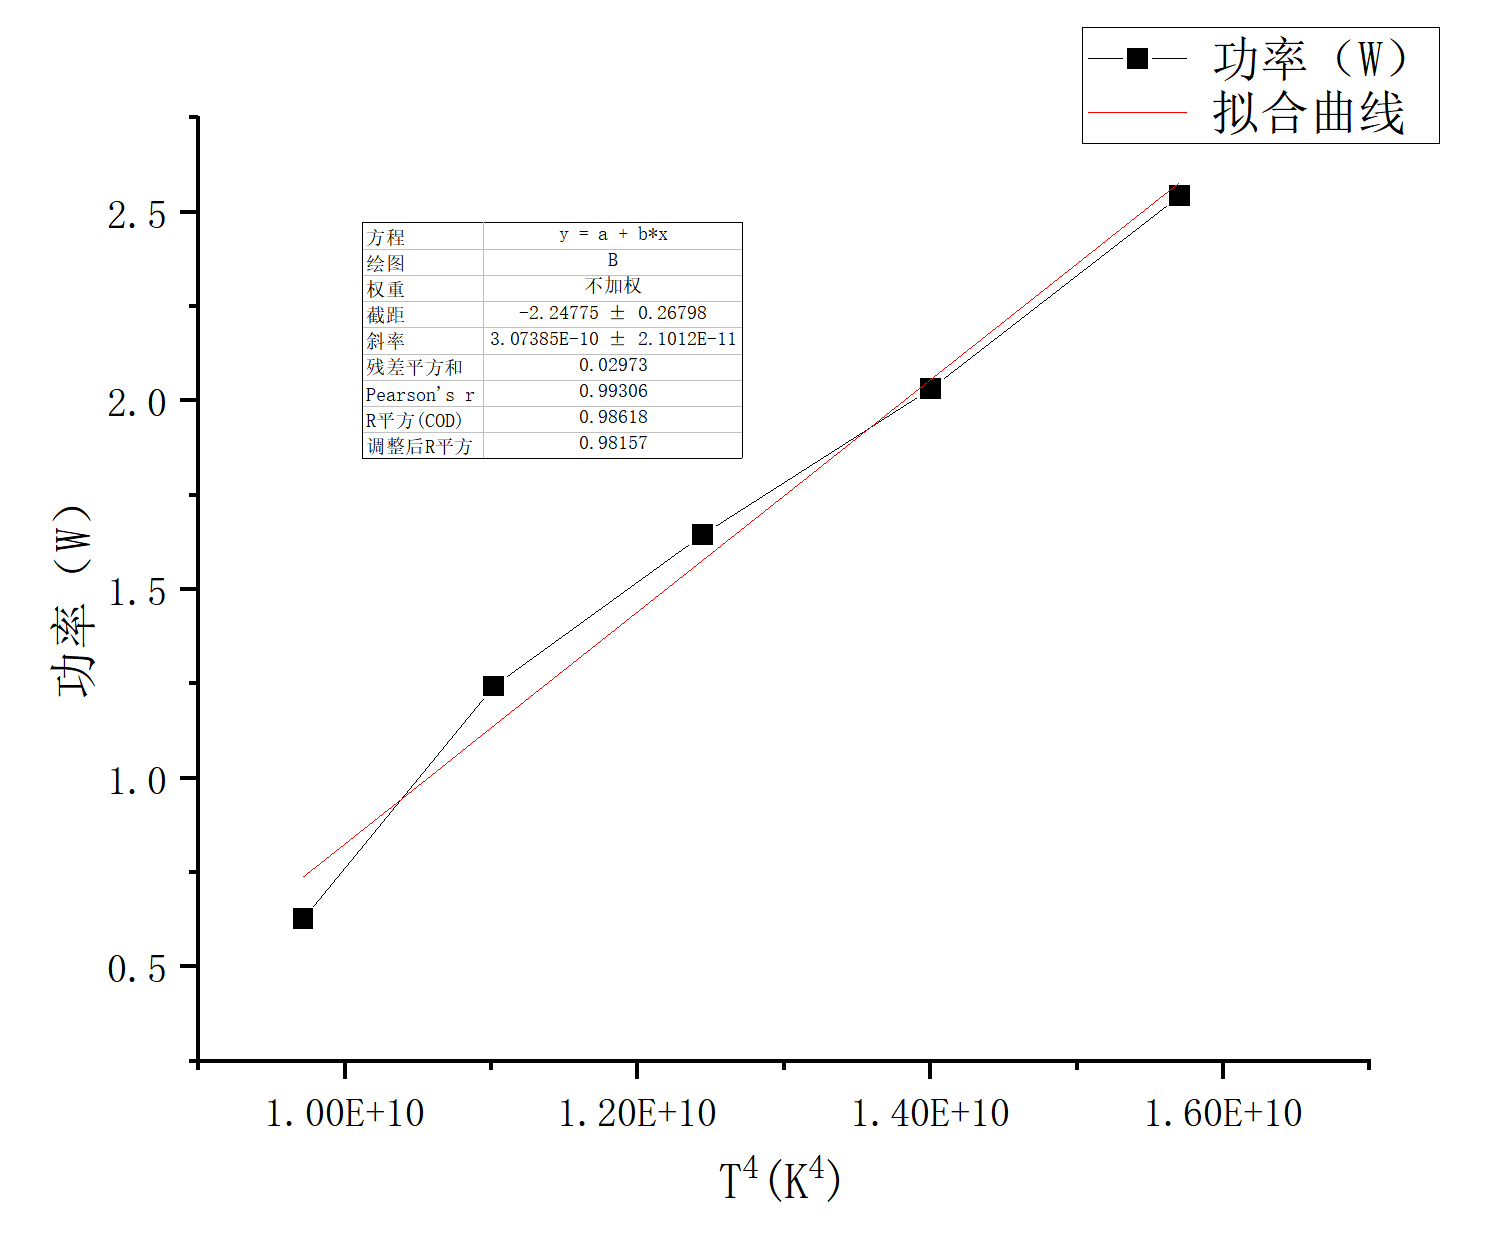
\includegraphics[width=0.6\linewidth]{功率拟合.png}
	\caption{电源加热功率与辐射体表面温度}
	\label{}
\end{figure}
\item 数据分析\\
    由图24可得,可见辐射强度与辐射体表面开氏温度的四次方成正比,即斯特藩-玻尔兹曼定律成立。\\
	根据拟合曲线的截距不为零说明拟合曲线并不过原点,这可能是由于实验过程中实验仪器可能会对热辐射产生影响,并且实验过程中空气可能会对实验数据产生影响,从而引入误差,并且由于横坐标的数值很大,可能会出现“失之毫厘谬以千里”的问题。\\
	尽管出现此种误差,但是根据$R^{2}=0.9985$可以判断,辐射传感器示数与表面温度的$T^4$成正比,斯特藩-玻尔兹曼定律成立。\\
    由图26可得,电源加热功率与辐射体表面温度成正比,$R^{2}=0.98618$,实验数据存在一定的误差,但是在误差允许范围之内,也符合实验预期,故可认定实验成功。

	\end{enumerate}
	
	%
	\subsubsection{测量在不同辐射距离在 d 的辐射传感器输出P,拟合给出$P-d$之间的关系}
	\begin{enumerate}
		\item 实验选取黑面样品进行测量,温度设定61℃进行实验,根据所得数据进行拟合。
		\begin{table}[!ht]
			\centering
			\begin{tabular}{|l|l|l|l|l|l|l|}
			\hline
				目标距离 d (mm) & 151 & 171 & 191 & 211 & 231 & 251  \\ \hline
				输出电压 P (µV )  & 407 & 282 & 224 & 174 & 147 & 119  \\ \hline
				$d^{-2}$& 4.38577E-05 & 3.41986E-05 & 2.74115E-05 & 2.24613E-05 & 1.87403E-05 & 1.58728E-05  \\ \hline
				
			\end{tabular}
		\end{table}
	
	
	\begin{figure}[{H}]
		\centering
		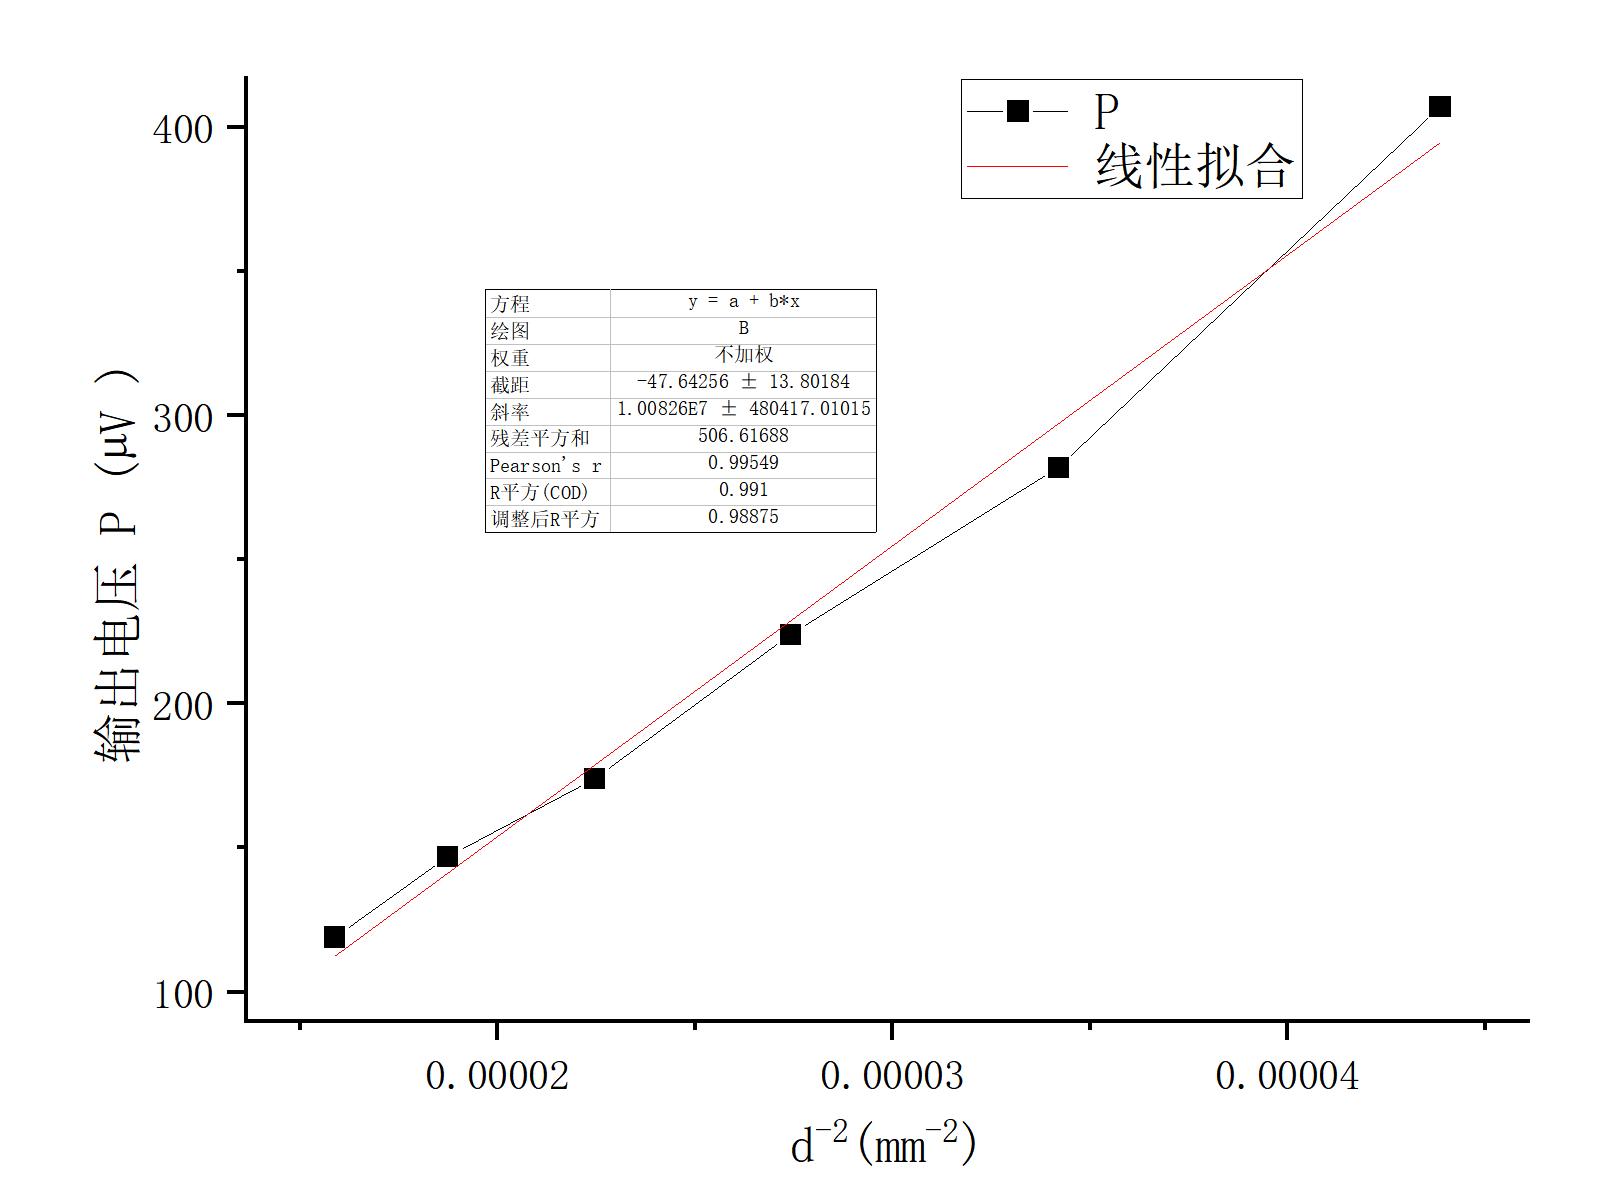
\includegraphics[width=0.6\linewidth]{d-2.png}
		\caption{$P-d^{-2}$拟合曲线}
		\label{}
	\end{figure}
	\item 数据分析\\
	$P-d^{-2}$曲线的$R^{2}=0.991$拟合效果很好,说明\textbf{具有类似光强和距离的平方成反比的规律}\\
	对比距离平方反比律与(平面辐射源的)辐射角关系式$$\dot{q}=\frac{\dot{q}_a}{2\pi}\int_0^{2\pi}d\omega\int_0^\alpha sin\theta cos\theta d\theta=\frac{\dot{q}_a}4(1-cos2\alpha)=\frac{\dot{q}_a}2sin^2\alpha $$
	根据此公式的推导过程,其与辐射面与接收器之间的所存在的张角有关,距离越近,张角显著增大,此时就不满足平方反比定律,\textbf{所以平方反比定律适用于距离较远的情况下,而辐射角关系式适用于较近的距离。}
	\item 对于思考题:以下距离的定义哪个正确:(1)从辐射表面到传感器表面(红外透镜)的距离;(2)从辐射表面到传感器内部热电堆表面的距离。\\
	\textbf{我认为第一种更正确,因为进入传感器表面的辐射大部分都会被吸收进仪器,所以此时可以认定进入的辐射即为最终辐射,如果此时再选择到内部为最终距离的话,会导致误差加剧。即对数据的要求是要在同一标准下,确定进入的辐射为最终辐射,那么则进入传感器的位置即为定义距离的位置,所以第一个定义是正确的。}\\
	他们对于误差的影响取决于传感器和辐射面之间的距离,距离越大,此种误差可以忽略,但是值得注意的是,由于在数据处理过程中存在平方反比的关系,所以会出现实验结果对于误差比较敏感,此时就要根据实验条件进行多组或者更高精度的测量。
	
	\end{enumerate}
	\subsubsection{测量不同物体表面的发射系数}
	设定温度为 61℃ 、距离为 150mm,分别使用黑面、粗面、光面样品进行实验,根据实验数据(表3)可知:
	$$\text{发射系数: 黑面>粗糙面>光面。}$$
	
	% ---
	
	% 实验后思考题
	\subsection{实验后思考题}
	
	%思考题1
	\begin{question}
		为何当热辐射传感器太靠近辐射表面时,所测出的辐照度偏离距离平方反比规律?
	\end{question}
	如上文所说,公式$\dot{q}=\frac{\dot{q}_a}2sin^2\alpha $与辐射面与接收器之间的所存在的张角有关,距离越近,张角显著增大,此时就不满足平方反比定律,\textbf{所以平方反比定律适用于距离较远的情况下,而辐射角关系式适用于较近的距离。}\\
	\indent 此外,辐射源表面可能存在非均匀性,例如局部温度变化或表面不平整,这会导致在距离辐射源较近的位置测量到的辐射强度与距离的平方反比关系不符。
	
	% 思考题2
	\begin{question}
	SMTIR9902与SMTIR9902SIL各有什么特点?各适合于什么场景的非接触温度测量?为什么?
	\end{question}
	SMTIR9902和SMTIR9902SIL是两款红外非接触式温度传感器,前者适用于一般环境中的温度测量,为过滤环境辐射的影响,增加了滤镜,以过滤可见光的影响,具有较高的精度和稳定性;而后者采用了SIL封装,则适用于高温高压环境,具有更好的耐热性和耐压性,能够稳定工作在恶劣的环境中。
	% 思考题3
	\begin{question}
	辐射传感器输出信号与辐射表面绝对温度4次方成线性关系,为何直线不过原点?斯特藩-玻尔兹曼定律是否成立?为什么?
	\end{question}
	正如数据分析时所写,此结果可能是由于误差引入导致的,这个误差可能是传感器本身的固有噪声、环境因素或者测量系统的校准误差等原因引起的,所以直线不过原点。\\
	此时斯特藩-玻尔兹曼定律仍然成立,这是由于尽管不过原点,但是直线拟合得非常好,$R^{2}=0.9985$,辐射传感器示数与表面温度的$T^4$成正比,斯特藩-玻尔兹曼定律成立。
	% ---
	要评估材料的防热辐射能力,需要考虑以下几个因素:
	\begin{question}
		如何评价材料(如透光隔热膜) 的防热辐射能力及其在窗户
应用中的节能效果?
		\end{question}
\begin{enumerate}
  \item \textbf{反射率}:材料的反射率指的是它对热辐射的反射能力。高反射率的材料能够将大部分的热辐射反射回去,减少吸收和热量传导。

  \item \textbf{吸收率}:吸收率表示材料吸收热辐射的能力。低吸收率的材料会较少吸收热量,因此能够保持较低的温度。

  \item \textbf{发射率}:发射率是指材料自身发出的热辐射相对于黑体的能力。低发射率的材料会减少热量的辐射,从而减少其自身的热量损失。

  \item \textbf{热传导}:热传导性指材料导热的能力。低热传导性的材料不容易传导热量,因此能够提高防热辐射能力。
  \item 窗户应用方面的节能效果:在窗户应用中,透光隔热膜可以有效减少太阳辐射和室内热量的进入,降低室内温度,提高舒适度。通过减少空调的使用,可以节省能源并降低能源消耗,从而达到节能的目的。同时,透光隔热膜还可以减少室内家具和地板等的日晒损坏,延长室内装饰的使用寿命。因此,透光隔热膜在窗户应用中具有显著的节能效果和环境保护作用。


\end{enumerate}
\begin{question}
	如何在(变化的)大气环境温度下测量各热辐射源的温度?
	\end{question}
	\begin{enumerate}
		\item \textbf{使用热像仪:} 热像仪可以直接测量热辐射源的红外辐射,而不受大气环境温度变化的影响。
	  
		\item \textbf{温度补偿方法:} 使用其他传感器来测量大气环境温度,并将其纳入到计算中,以便修正测量结果。
	  
		\item \textbf{控制环境条件:} 尽可能在室内进行测量,并考虑使用隔热罩或屏蔽物来减少外部环境的影响。
	  
		\item \textbf{多次测量和平均处理:} 进行多次测量,并对结果进行平均处理,可以减少测量误差,并提高测量结果的准确性。
	  \end{enumerate}
	
	% 结语部分
	\clearpage
	
	% 小标题
	\section{CC1 热辐射的测量\quad\heiti 结语}
	% ---
	
	% 总结、杂谈与致谢
	\subsection{实验心得和体会}
	\begin{enumerate}
		\item 实验总体难度不大,只要理解了实验原理就可以很快速的完成实验
		\item 实验重点在于要正确接线,有些情况实验仪器可能与示意图不相符,此时需要自行进行分析,得出正确的实验接线。
		\item 实验过程需要细心,提前做好预习,例如我在完成预习之后就决定在61℃完成后续实验,完成后再进行升温,这样就剩去了等待仪器降温的时间。
	\end{enumerate}
	% ---
	

	% 附件
	\subsection{附件及实验相关的软硬件资料等}
	
	\begin{figure}[{H}]
		\centering
		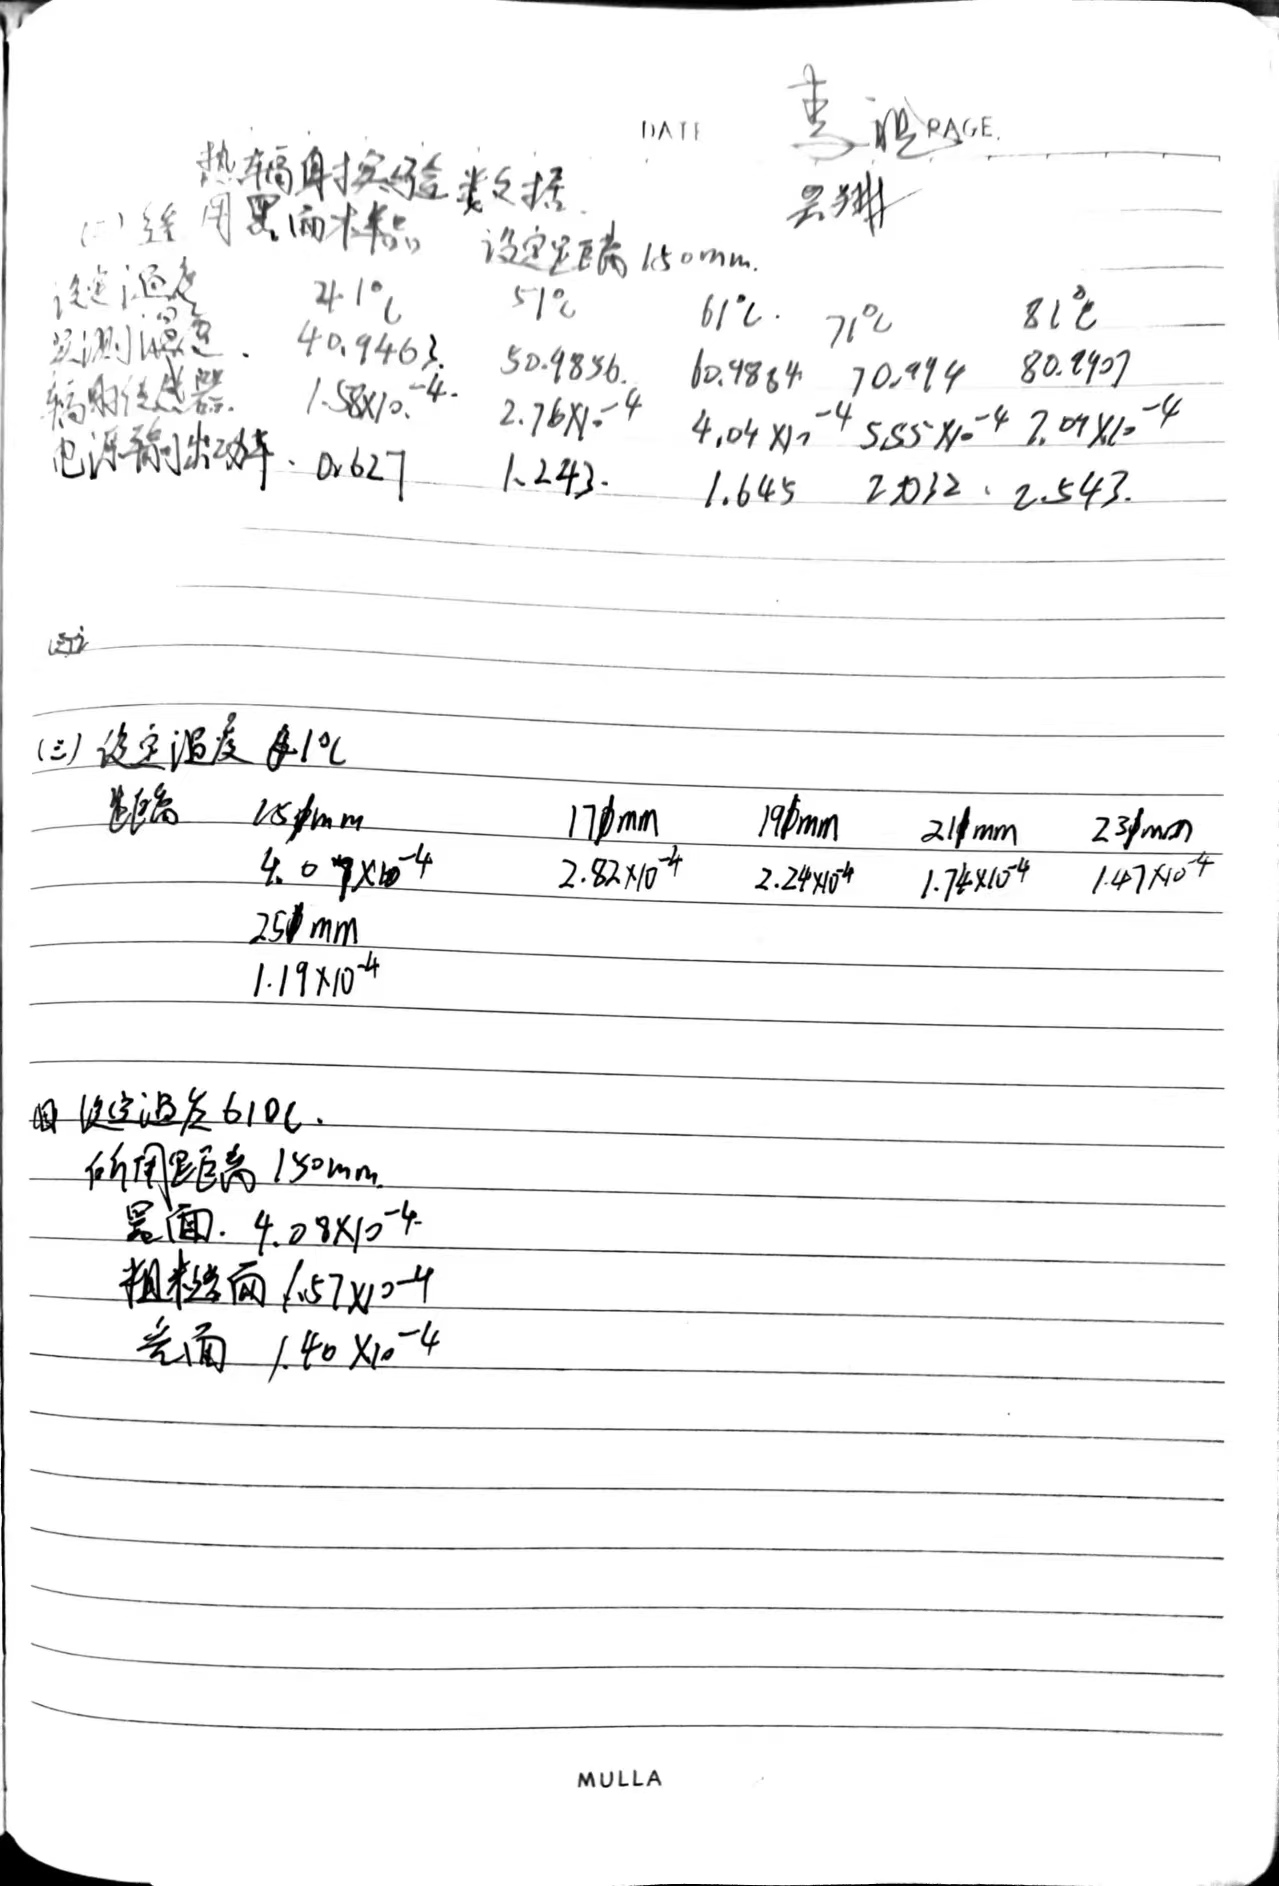
\includegraphics[width=0.3\linewidth]{原始数据.jpg}
		\caption{实验原始数据及签字}
		\label{}
	\end{figure}
	\begin{figure}[{H}]
		\centering
		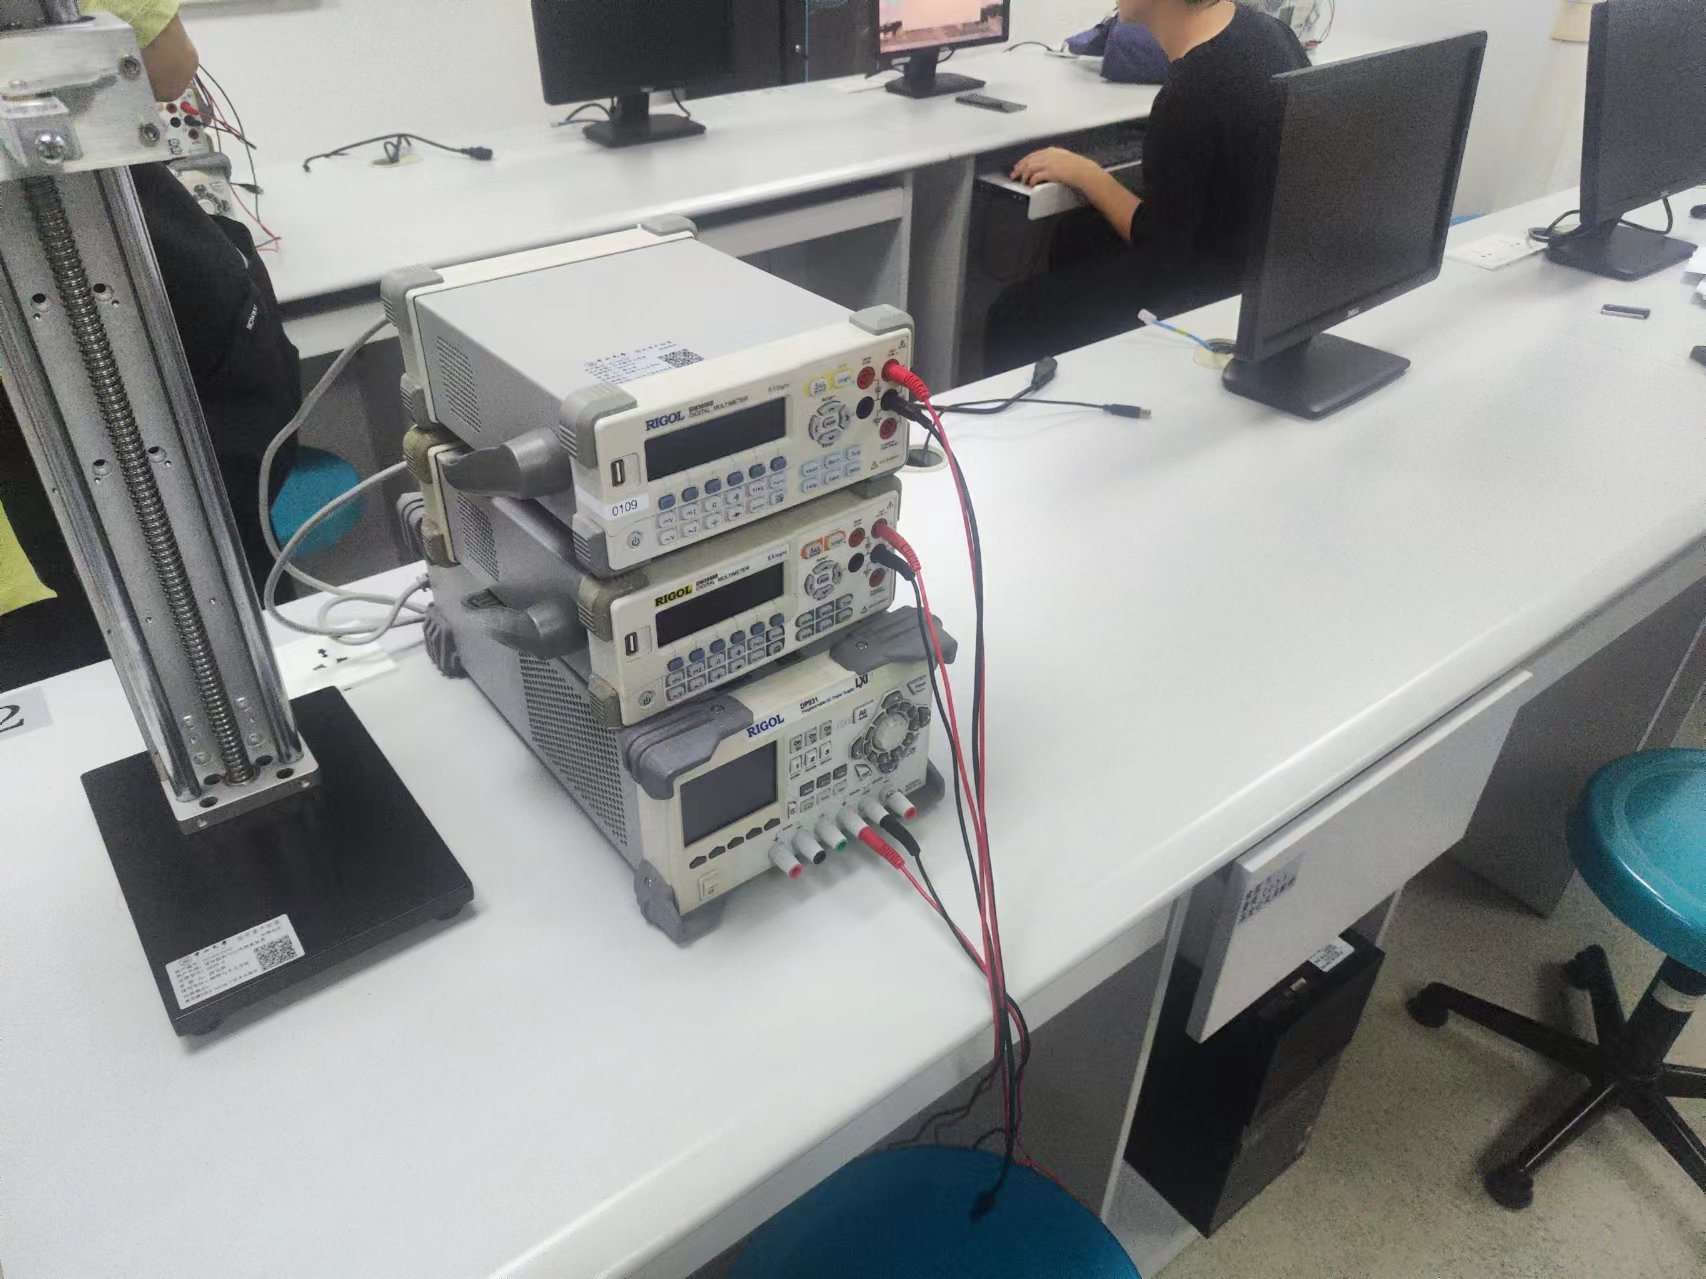
\includegraphics[width=0.4\linewidth]{桌面.jpg}
		\caption{实验桌面整理}
		\label{}
	\end{figure}
\end{document}